
\documentclass[12pt,a4paper]{article}

\setlength{\topmargin}{0.0in}
\setlength{\oddsidemargin}{0.33in}
\setlength{\textheight}{9.0in}
\setlength{\textwidth}{6.0in}
\renewcommand{\baselinestretch}{1.25}

\usepackage{nicematrix}
\usepackage[margin=0.75in]{geometry}
\usepackage[edges]{forest}
\usepackage{graphicx,wrapfig,lipsum}
\usepackage{amsmath,empheq}
\usepackage{dirtree}
\usepackage{titlesec}
\setcounter{secnumdepth}{4}
\titleformat{\paragraph}
{\normalfont\normalsize\bfseries}{\theparagraph}{1em}{}
\titlespacing*{\paragraph}
{0pt}{3.25ex plus 1ex minus .2ex}{1.5ex plus .2ex}
\usepackage{amssymb}
\usepackage{amsthm}
\usepackage[style=numeric,backend=biber]{biblatex}
\addbibresource{bibliography.bib}
\usepackage{tikz}
\def\checkmark{\tikz\fill[scale=0.4](0,.35) -- (.25,0) -- (1,.7) -- (.25,.15) -- cycle;}
\usepackage[utf8]{inputenc}
\usepackage[english]{babel}
\usepackage{hyperref}
\usepackage[ruled]{algorithm2e}
\usepackage{amssymb}
\usepackage{graphicx}
\usepackage{cancel}
\usepackage{epstopdf}
\usepackage{mathtools}
\usepackage{float}
\usepackage{caption}
\usepackage{subcaption}
\usepackage{setspace}
\usepackage{bm}
\usepackage[export]{adjustbox}
\usepackage{relsize}
\usepackage{listings}
\usepackage[toc,page]{appendix}
\usepackage{cancel}
\usepackage{color} %red, green, blue, yellow, cyan, magenta, black, white

\title{Gaffney Monk 2006}
\author{}

\begin{document}
\maketitle
\thispagestyle{empty}
\newpage
\setcounter{page}{1}
\newpage

\subsection{$\tau=0$}
\begin{figure}[H]
    \centering
    \begin{subfigure}[b]{0.45\linewidth}
        \centering
        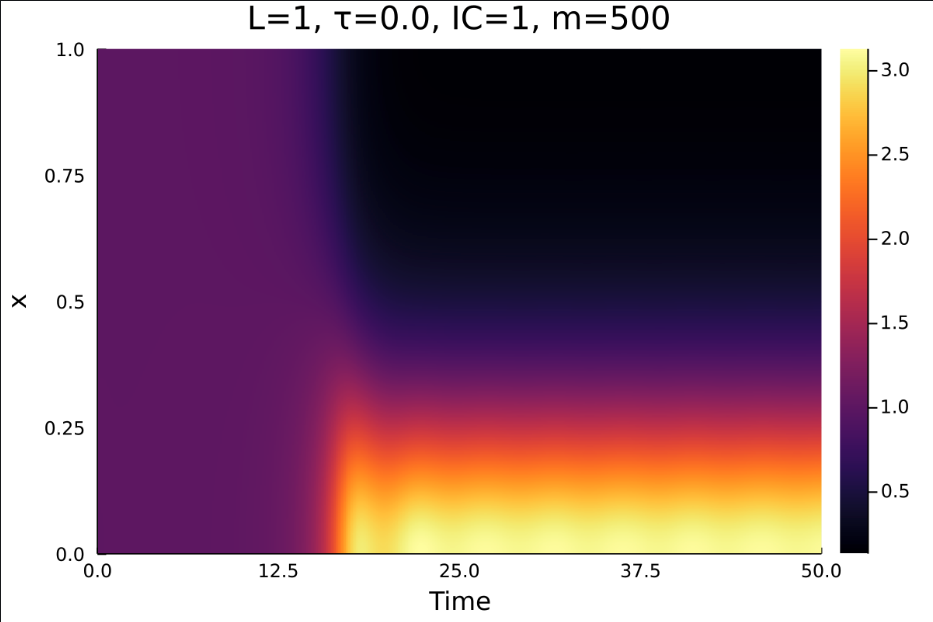
\includegraphics[width=6cm,height = 4.5cm]{l1t0ic1.png}
        \caption{}
        \label{}
    \end{subfigure}
    \hfill
    \begin{subfigure}[b]{0.45\linewidth}
        \centering
        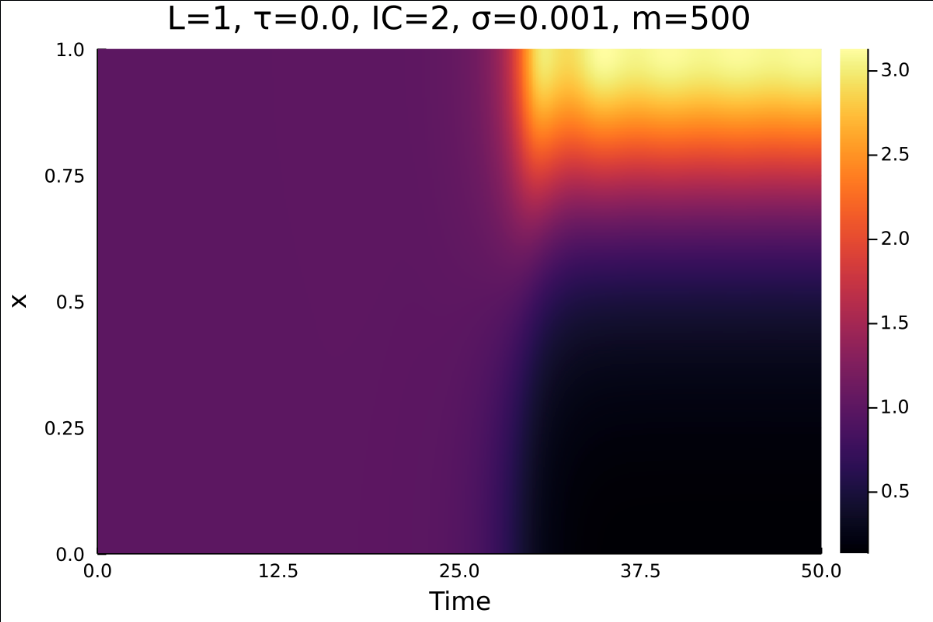
\includegraphics[width=6cm,height = 4.5cm]{l1t0ic2s1e3.png}
        \caption{}
        \label{}
    \end{subfigure}
    \hfill
    \begin{subfigure}[b]{0.45\linewidth}
        \centering
        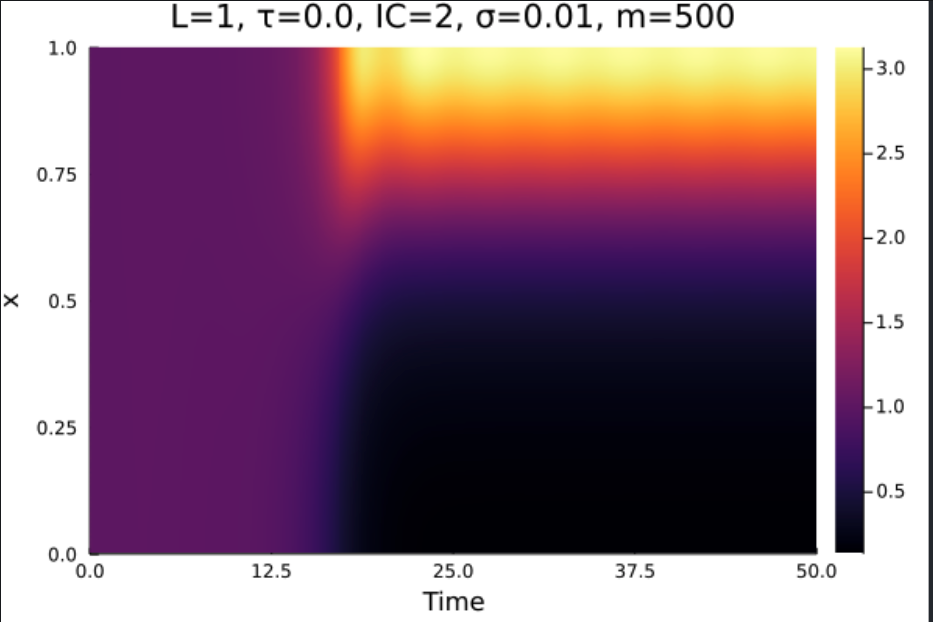
\includegraphics[width=6cm,height = 4.5cm]{l1t0ic2s1e2.png}
        \caption{}
        \label{}
    \end{subfigure}
    \hfill
    \begin{subfigure}[b]{0.45\linewidth}
        \centering
        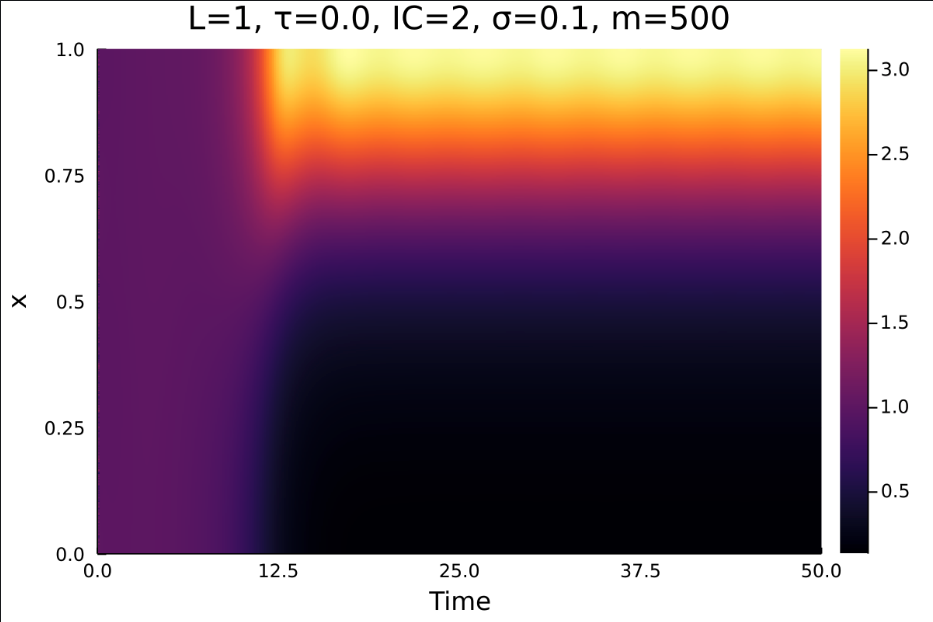
\includegraphics[width=6cm,height = 4.5cm]{l1t0ic2s1e1.png}
        \caption{}
        \label{}
    \end{subfigure}
    \caption{Results for $\tau=0$, $L=1$}
    \label{}
\end{figure}

\begin{figure}[H]
    \centering
    \begin{subfigure}[b]{0.45\linewidth}
        \centering
        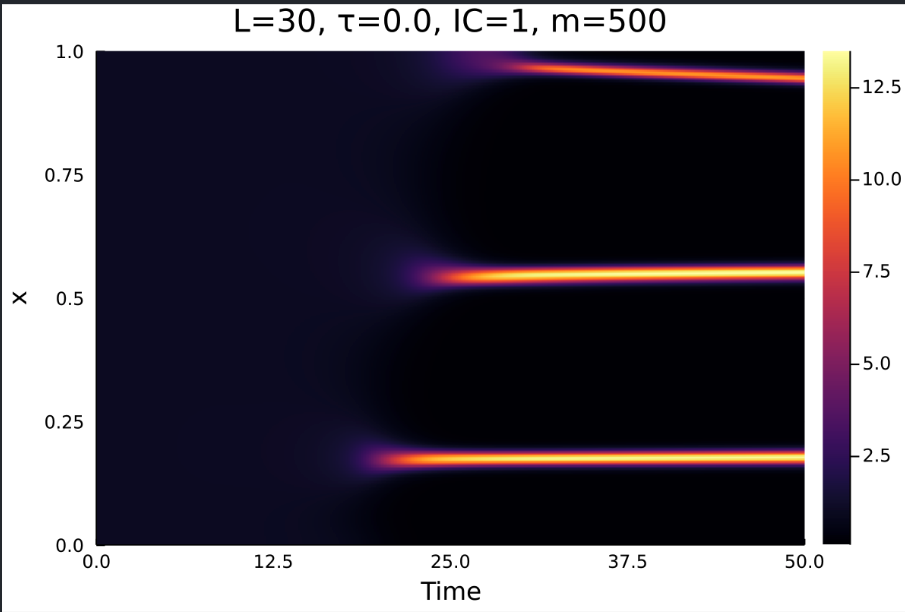
\includegraphics[width=6cm,height = 4.5cm]{l30t0ic1.png}
        \caption{}
        \label{}
    \end{subfigure}
    \hfill
    \begin{subfigure}[b]{0.45\linewidth}
        \centering
        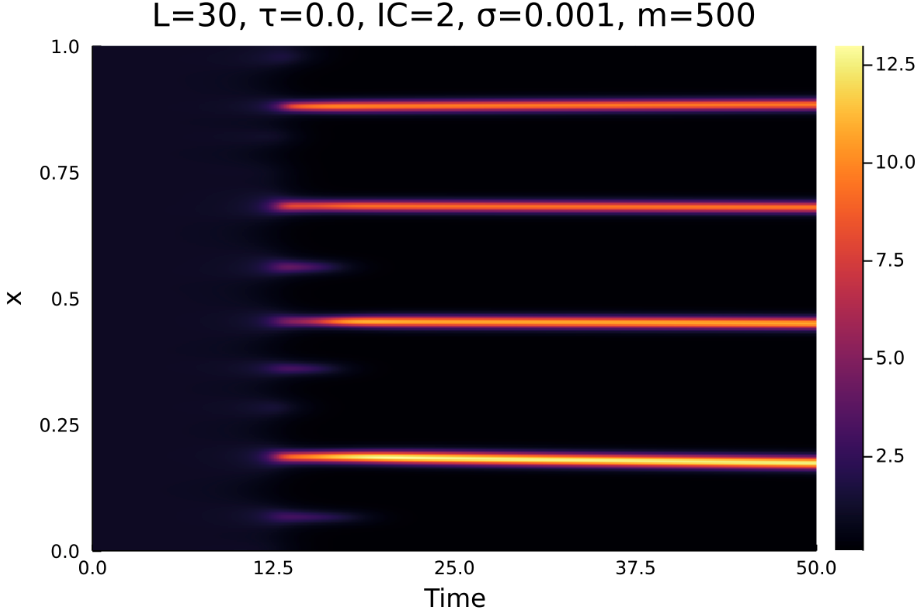
\includegraphics[width=6cm,height = 4.5cm]{l30t0ic2s1e3.png}
        \caption{}
        \label{}
    \end{subfigure}
    \hfill
    \begin{subfigure}[b]{0.45\linewidth}
        \centering
        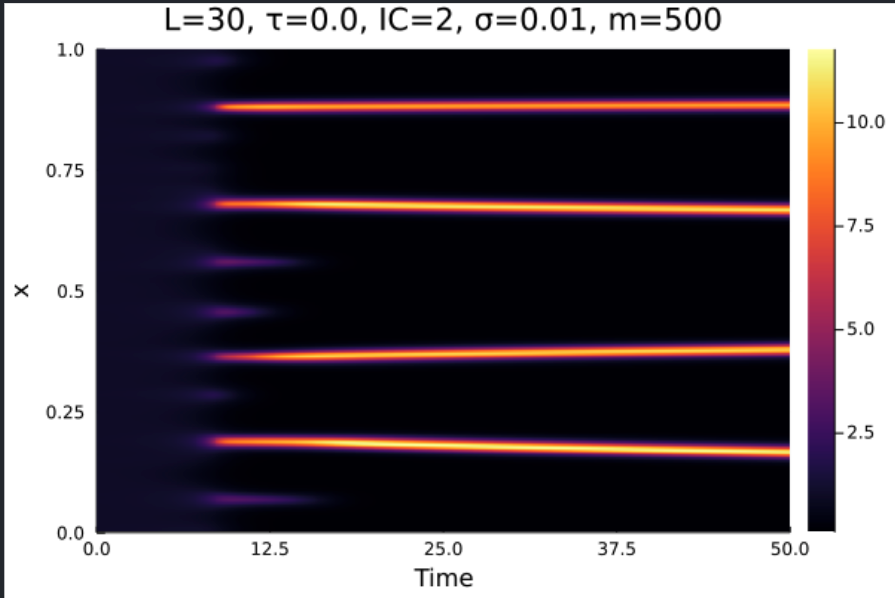
\includegraphics[width=6cm,height = 4.5cm]{l30t0ic2s1e2.png}
        \caption{}
        \label{}
    \end{subfigure}
    \hfill
    \begin{subfigure}[b]{0.45\linewidth}
        \centering
        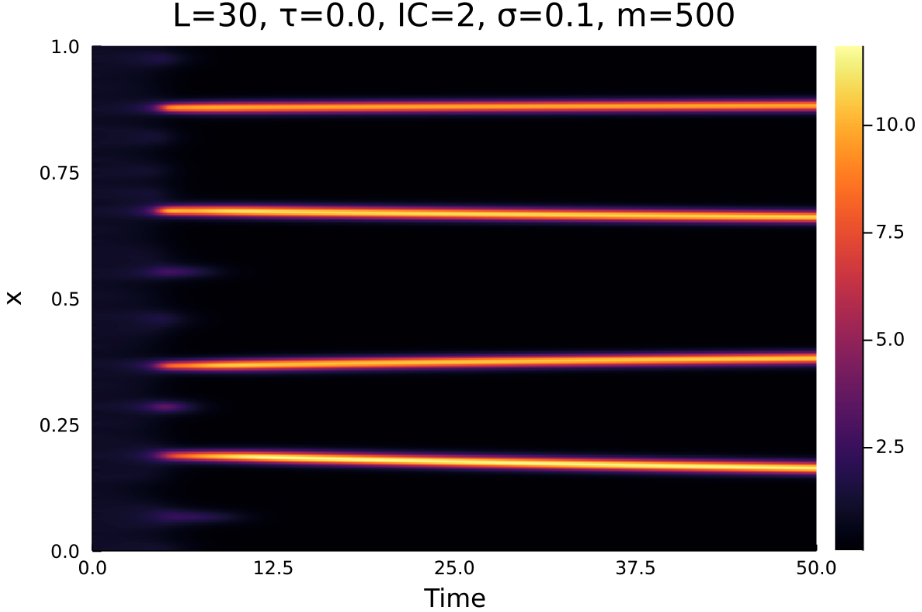
\includegraphics[width=6cm,height = 4.5cm]{l30t0ic2s1e1.png}
        \caption{}
        \label{}
    \end{subfigure}
    \caption{Results for $\tau=0$, $L=30$.}
    \label{}
\end{figure}










\subsection{$\tau=1$}


\begin{figure}[H]
    \centering
    \begin{subfigure}[b]{0.45\linewidth}
        \centering
        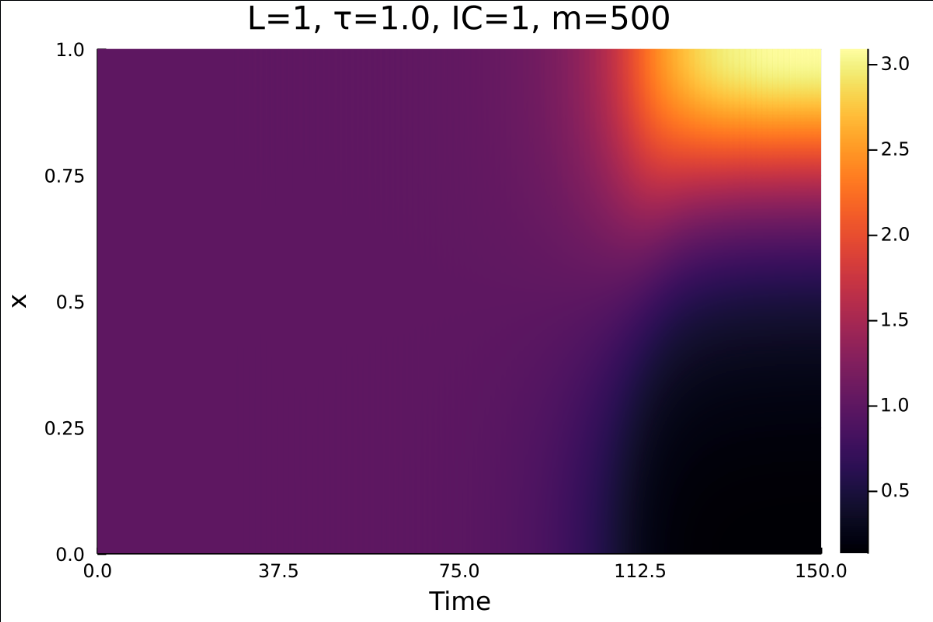
\includegraphics[width=6cm,height = 4.5cm]{l1t1ic1.png}
        \caption{}
        \label{}
    \end{subfigure}
    \hfill
    \begin{subfigure}[b]{0.45\linewidth}
        \centering
        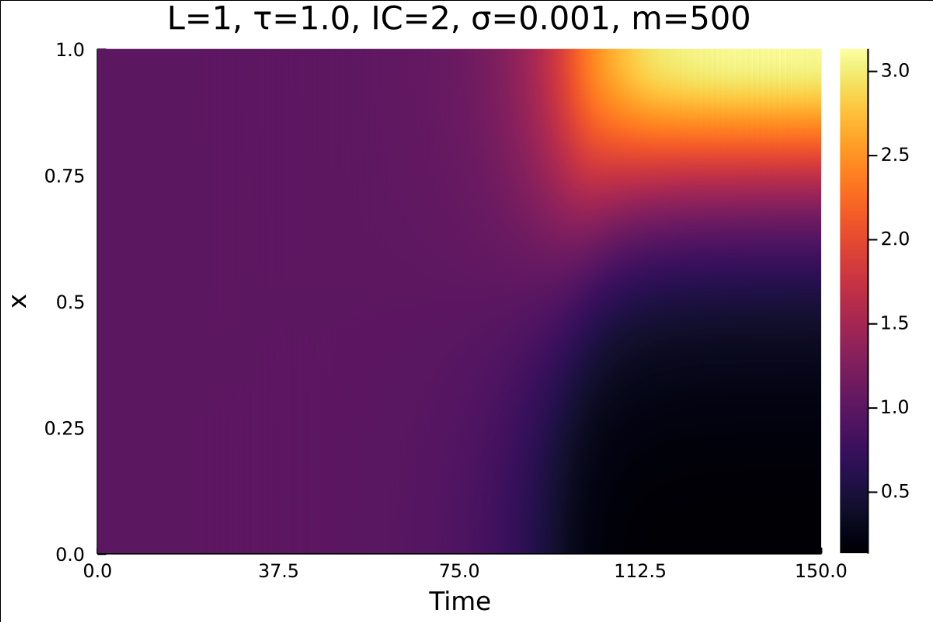
\includegraphics[width=6cm,height = 4.5cm]{l1t1ic2s1e3.png}
        \caption{}
        \label{}
    \end{subfigure}
    \hfill
    \begin{subfigure}[b]{0.45\linewidth}
        \centering
        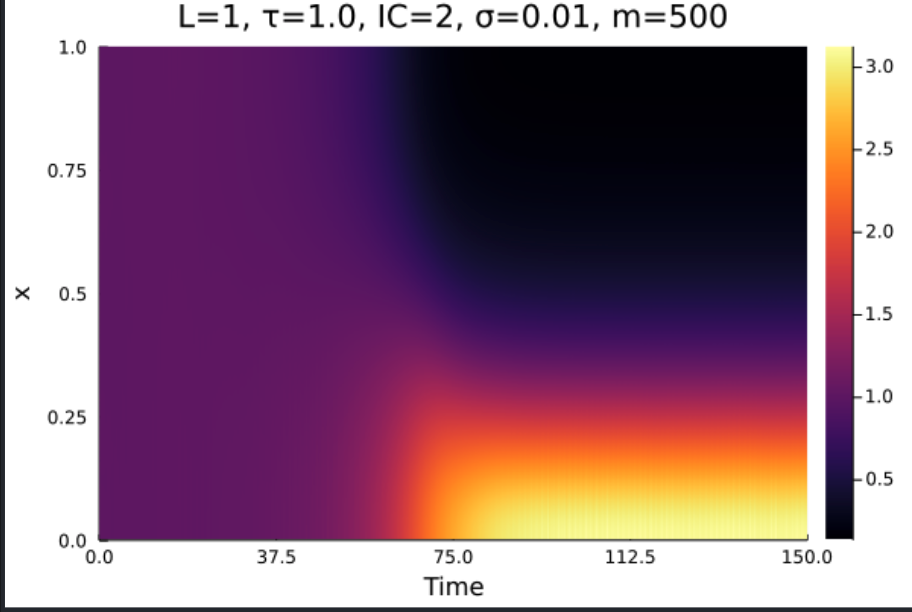
\includegraphics[width=6cm,height = 4.5cm]{l1t1ic2s1e2.png}
        \caption{}
        \label{}
    \end{subfigure}
    \hfill
    \begin{subfigure}[b]{0.45\linewidth}
        \centering
        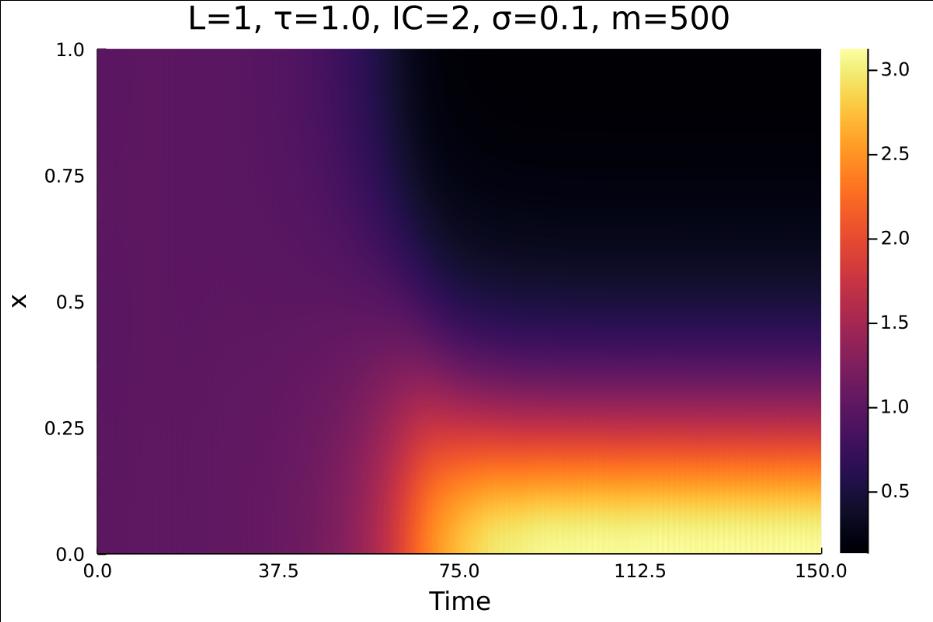
\includegraphics[width=6cm,height = 4.5cm]{l1t1ic2s1e1.png}
        \caption{}
        \label{}
    \end{subfigure}
    \caption{Results for $\tau=1$, $L=1$}
    \label{}
\end{figure}

\begin{figure}[H]
    \centering
    \begin{subfigure}[b]{0.45\linewidth}
        \centering
        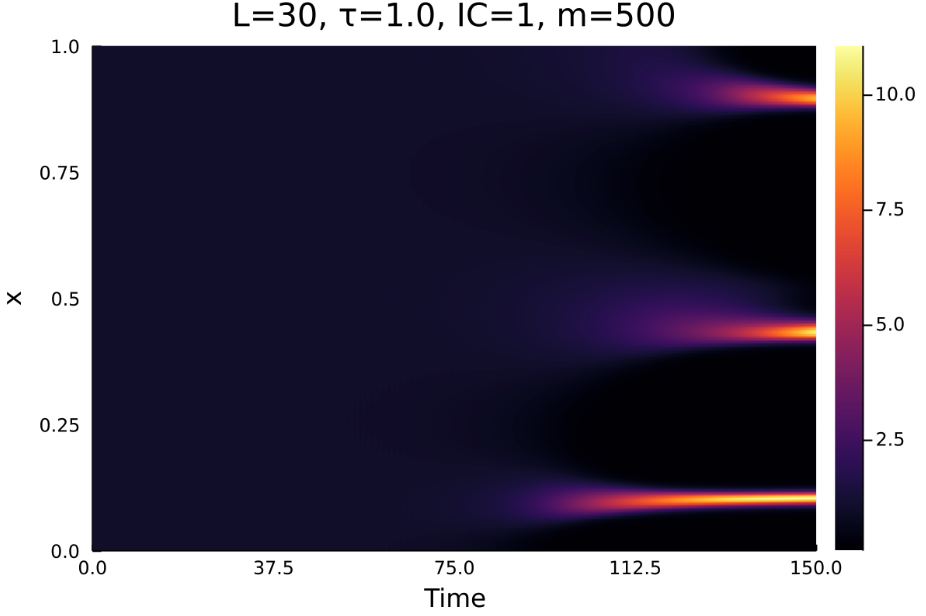
\includegraphics[width=6cm,height = 4.5cm]{l30t1ic1.png}
        \caption{}
        \label{}
    \end{subfigure}
    \hfill
    \begin{subfigure}[b]{0.45\linewidth}
        \centering
        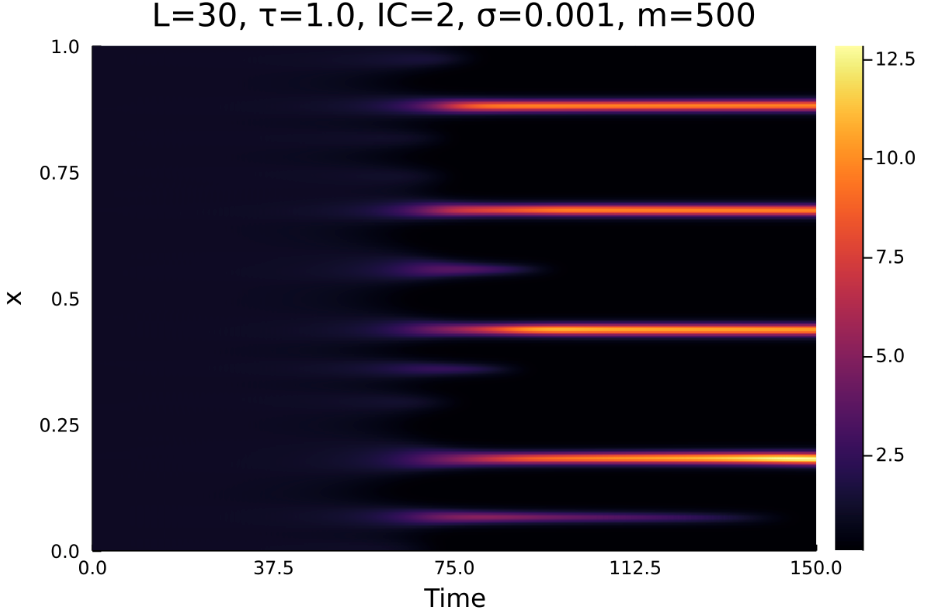
\includegraphics[width=6cm,height = 4.5cm]{l30t1ic2s1e3.png}
        \caption{}
        \label{}
    \end{subfigure}
    \hfill
    \begin{subfigure}[b]{0.45\linewidth}
        \centering
        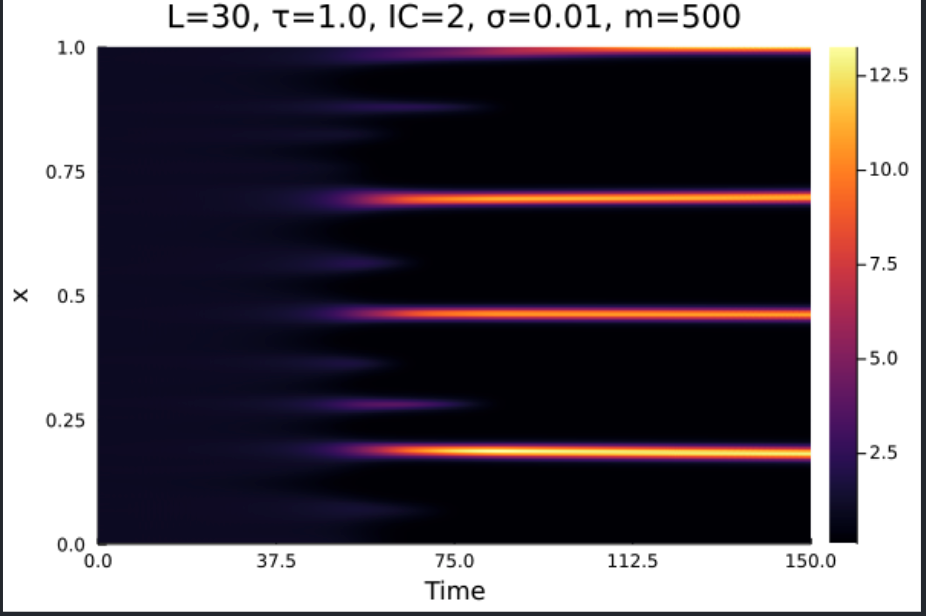
\includegraphics[width=6cm,height = 4.5cm]{l30t1ic2s1e2.png}
        \caption{}
        \label{}
    \end{subfigure}
    \hfill
    \begin{subfigure}[b]{0.45\linewidth}
        \centering
        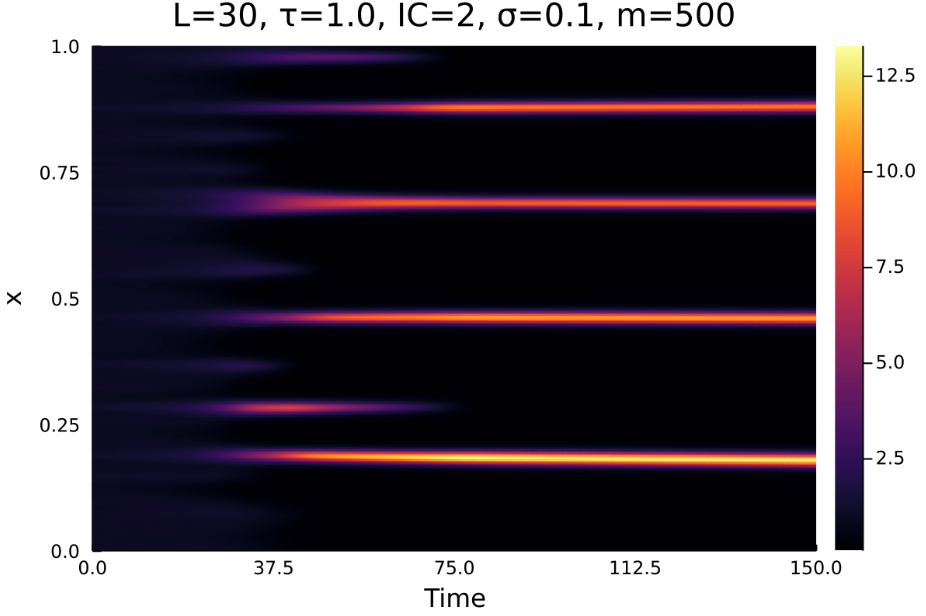
\includegraphics[width=6cm,height = 4.5cm]{l30t1ic2s1e1.png}
        \caption{}
        \label{}
    \end{subfigure}
    \caption{Results for $\tau=1$, $L=30$}
    \label{}
\end{figure}






\subsection{$\tau=2$}
\begin{figure}[H]
    \centering
    \begin{subfigure}[b]{0.45\linewidth}
        \centering
        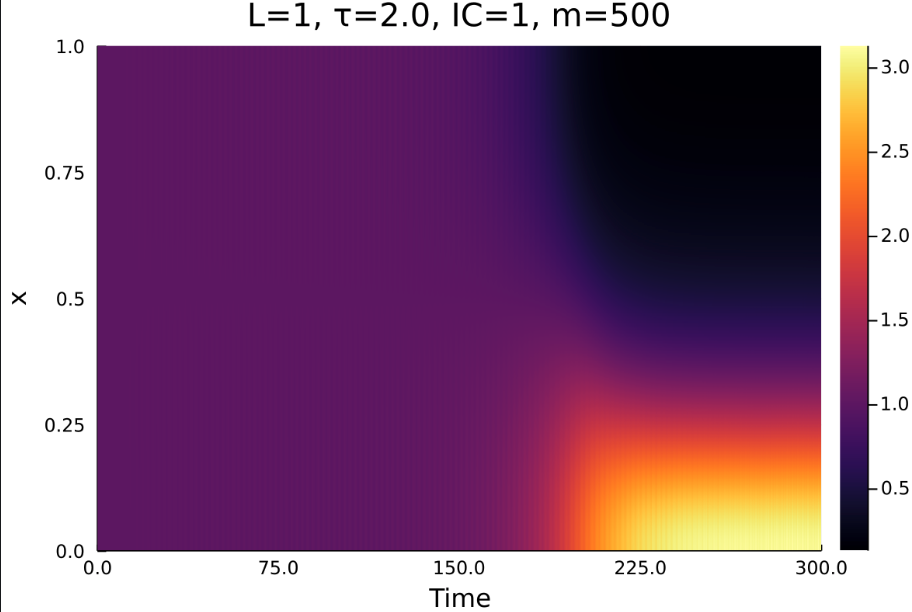
\includegraphics[width=6cm,height = 4.5cm]{l1t2ic1.png}
        \caption{}
        \label{}
    \end{subfigure}
    \hfill
    \begin{subfigure}[b]{0.45\linewidth}
        \centering
        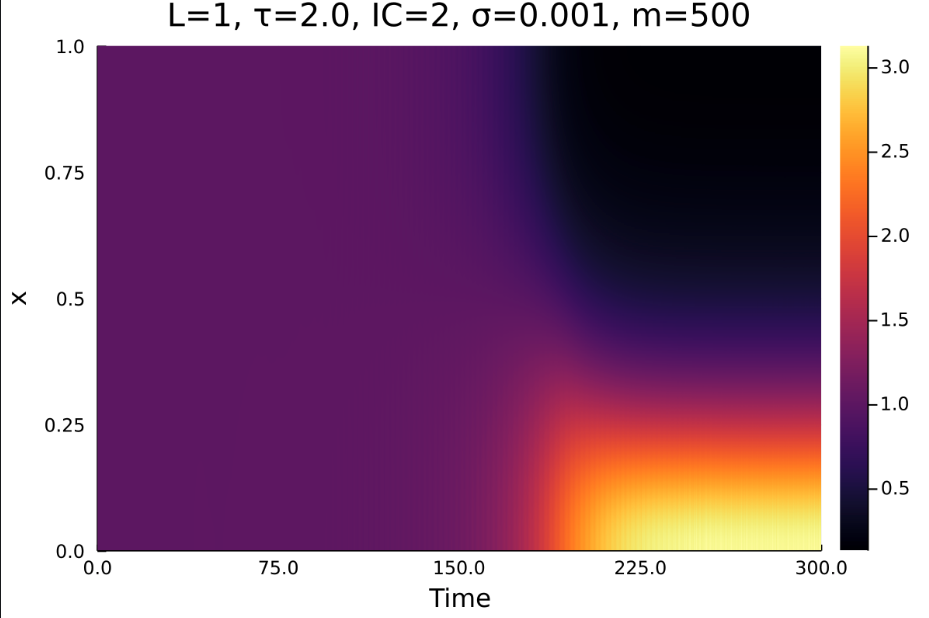
\includegraphics[width=6cm,height = 4.5cm]{l1t2ic2s1e3.png}
        \caption{}
        \label{}
    \end{subfigure}
    \hfill
    \begin{subfigure}[b]{0.45\linewidth}
        \centering
        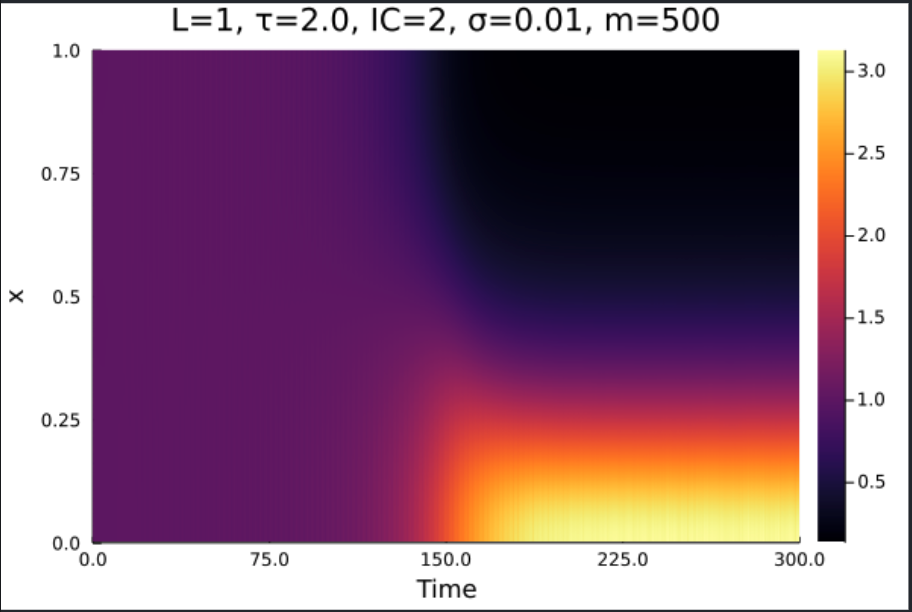
\includegraphics[width=6cm,height = 4.5cm]{l1t2ic2s1e2.png}
        \caption{}
        \label{}
    \end{subfigure}
    \hfill
    \begin{subfigure}[b]{0.45\linewidth}
        \centering
        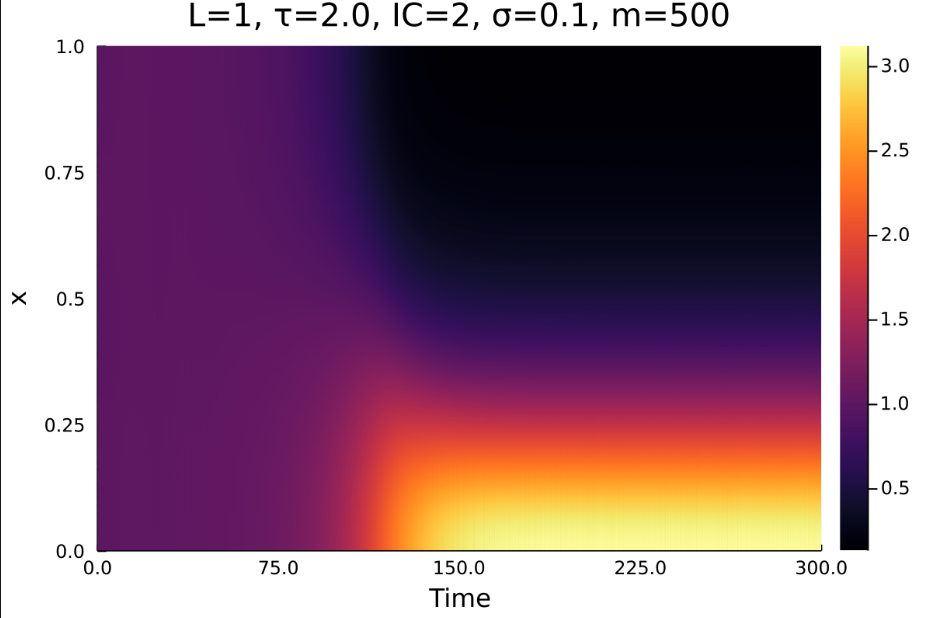
\includegraphics[width=6cm,height = 4.5cm]{l1t2ic2s1e1.png}
        \caption{}
        \label{}
    \end{subfigure}
    \caption{Results for $\tau=2$}
    \label{}
\end{figure}

\begin{figure}[H]
    \centering
    \begin{subfigure}[b]{0.45\linewidth}
        \centering
        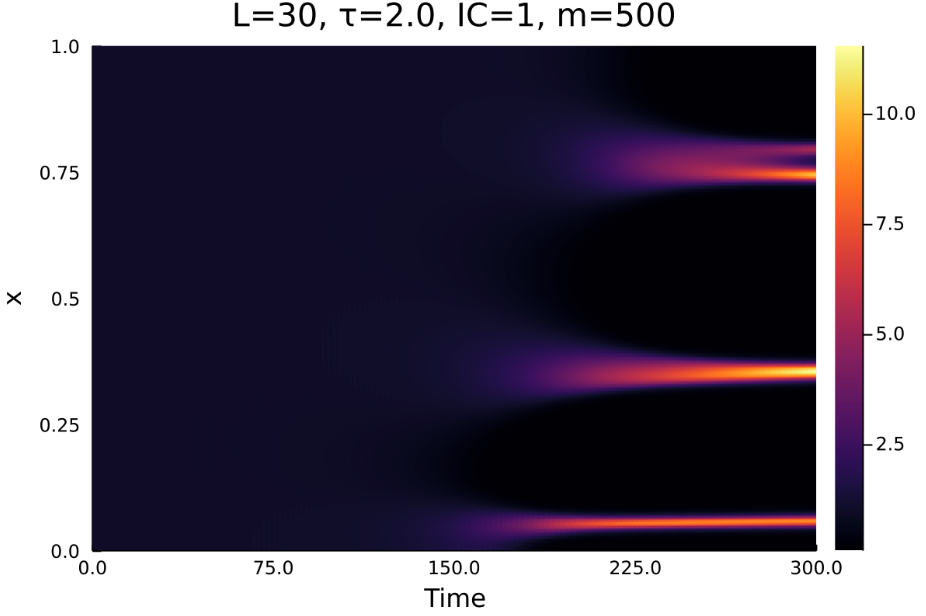
\includegraphics[width=6cm,height = 4.5cm]{l30t2ic1.png}
        \caption{}
        \label{}
    \end{subfigure}
    \hfill
    \begin{subfigure}[b]{0.45\linewidth}
        \centering
        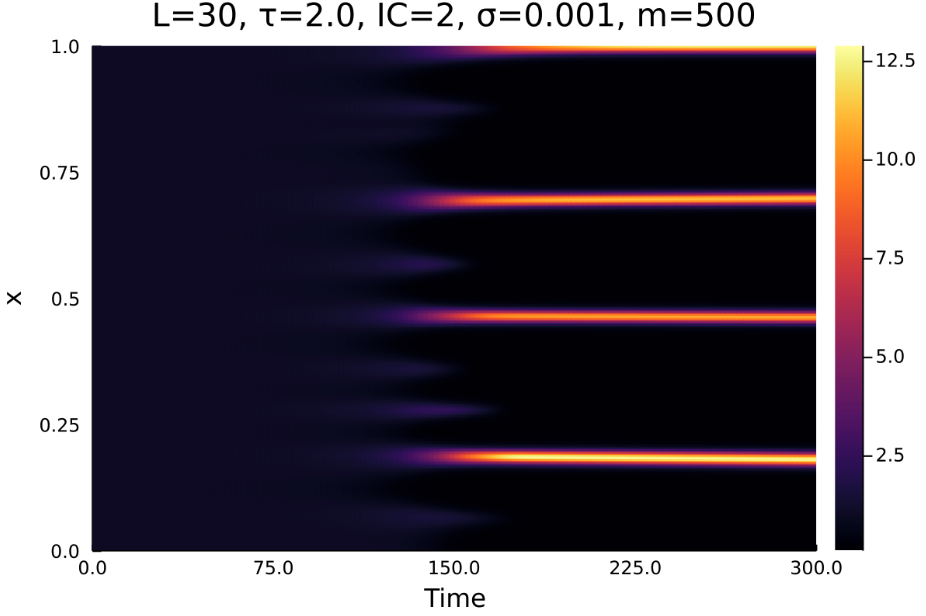
\includegraphics[width=6cm,height = 4.5cm]{l30t2ic2s1e3.png}
        \caption{}
        \label{}
    \end{subfigure}
    \hfill
    \begin{subfigure}[b]{0.45\linewidth}
        \centering
        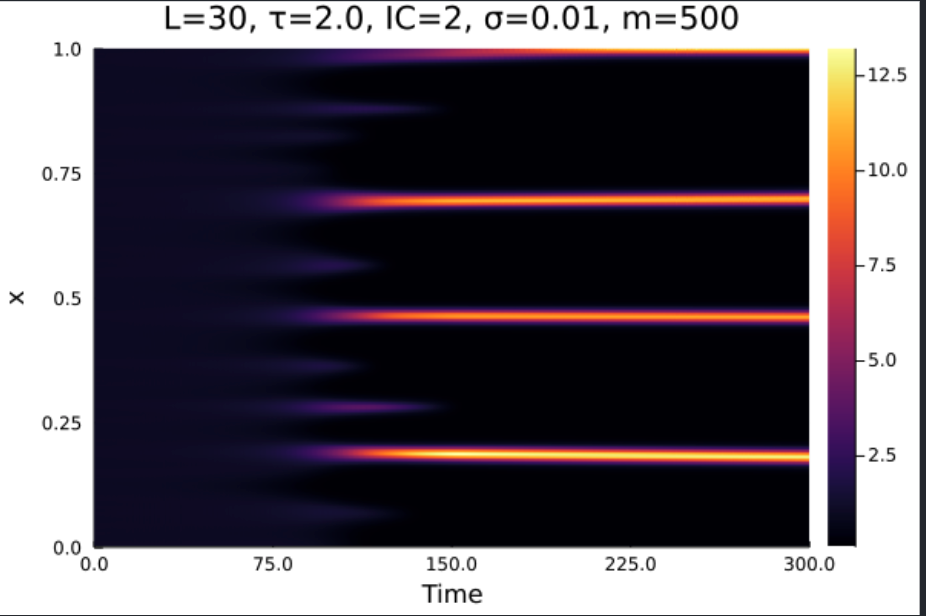
\includegraphics[width=6cm,height = 4.5cm]{l30t2ic2s1e2.png}
        \caption{}
        \label{}
    \end{subfigure}
    \hfill
    \begin{subfigure}[b]{0.45\linewidth}
        \centering
        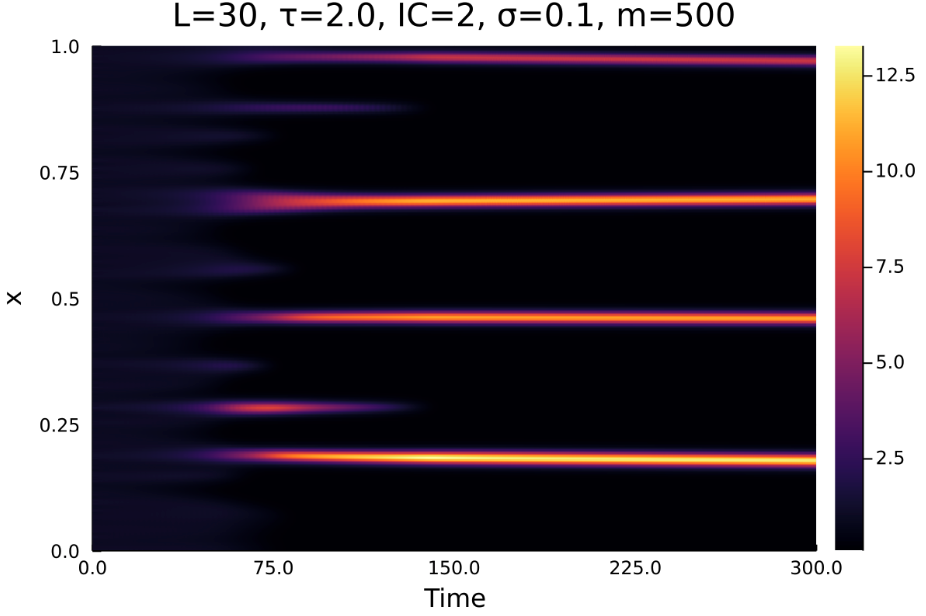
\includegraphics[width=6cm,height = 4.5cm]{l30t2ic2s1e1.png}
        \caption{}
        \label{}
    \end{subfigure}
    \caption{Results for $\tau=2$}
    \label{}
\end{figure}


\subsection{Introducing variation in history}


\begin{figure}[H]
    \begin{subfigure}[b]{0.45\linewidth}
        \centering
        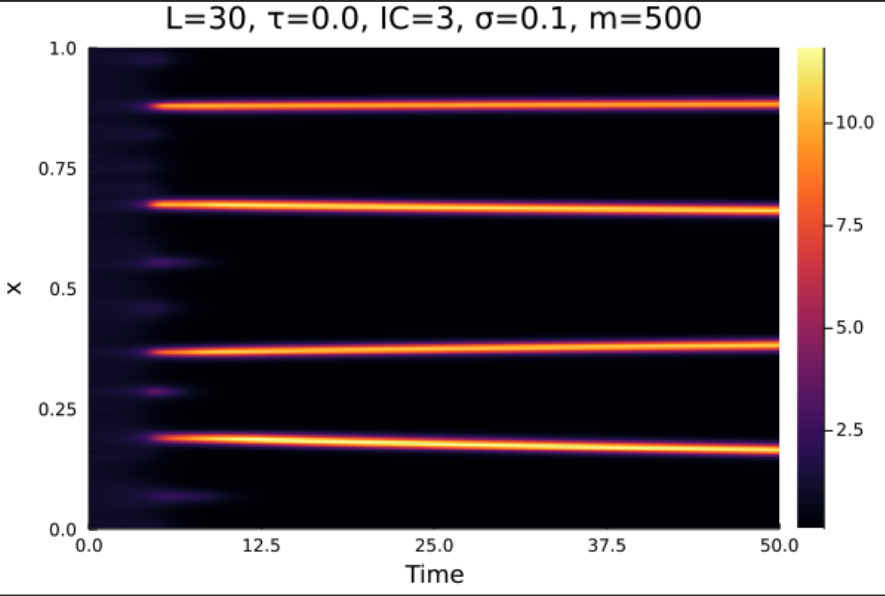
\includegraphics[width=6cm,height = 4.5cm]{l30t0ic3s1e1.png}
        \caption{}
        \label{}
    \end{subfigure}
    \hfill
    \begin{subfigure}[b]{0.45\linewidth}
        \centering
        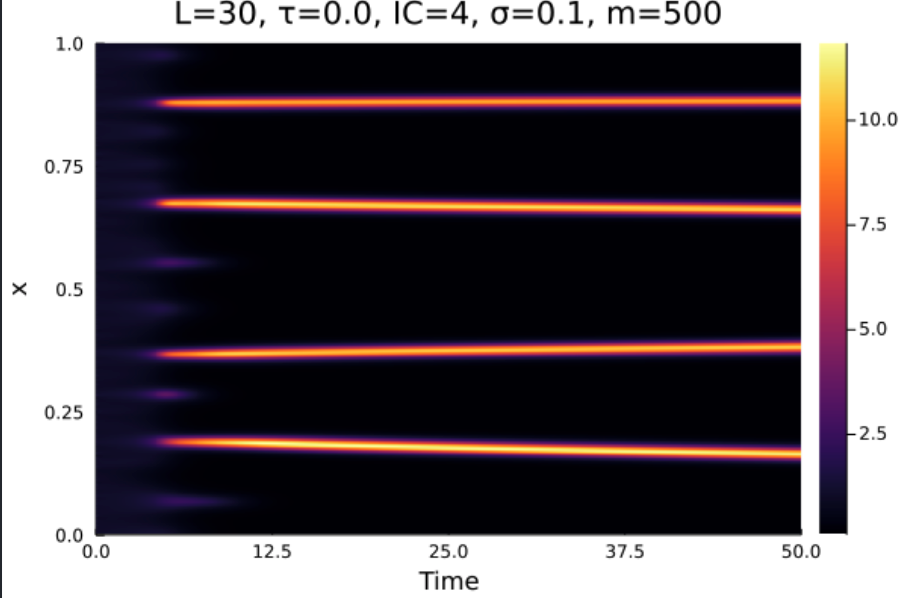
\includegraphics[width=6cm,height = 4.5cm]{l30t0ic4s1e1.png}
        \caption{}
        \label{}
    \end{subfigure}
    \newline
    \hfill
    \begin{subfigure}[b]{0.45\linewidth}
        \centering
        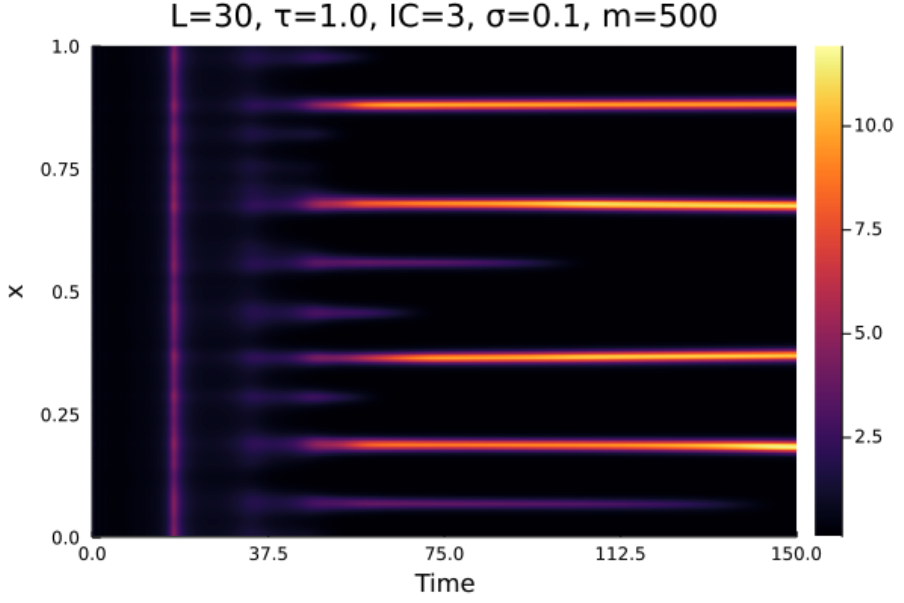
\includegraphics[width=6cm,height = 4.5cm]{l30t1ic3s1e1.png}
        \caption{}
        \label{}
    \end{subfigure}
    \hfill
    \begin{subfigure}[b]{0.45\linewidth}
        \centering
        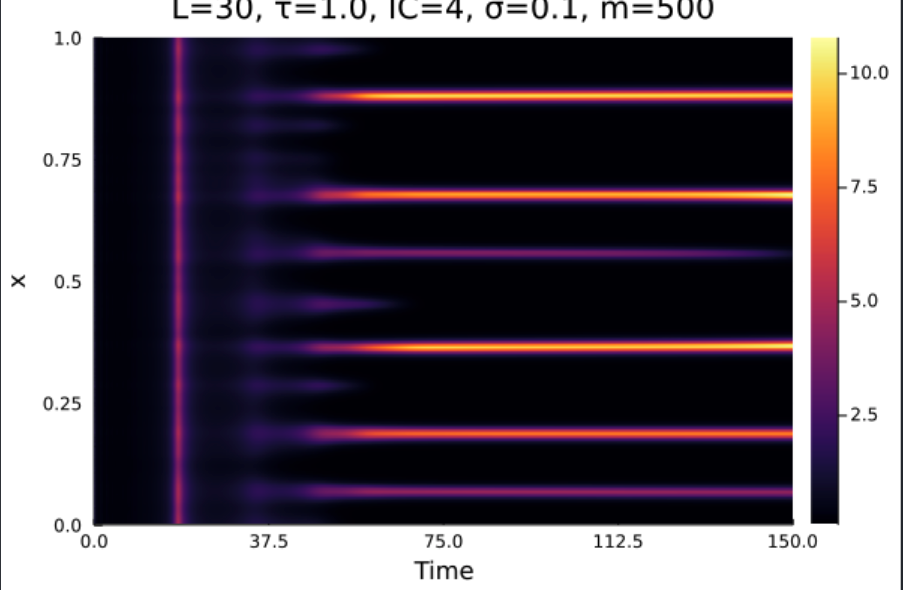
\includegraphics[width=6cm,height = 4.5cm]{l30t1ic4s1e1.png}
        \caption{}
        \label{}
    \end{subfigure}
    \hfill
    \begin{subfigure}[b]{0.45\linewidth}
        \centering
        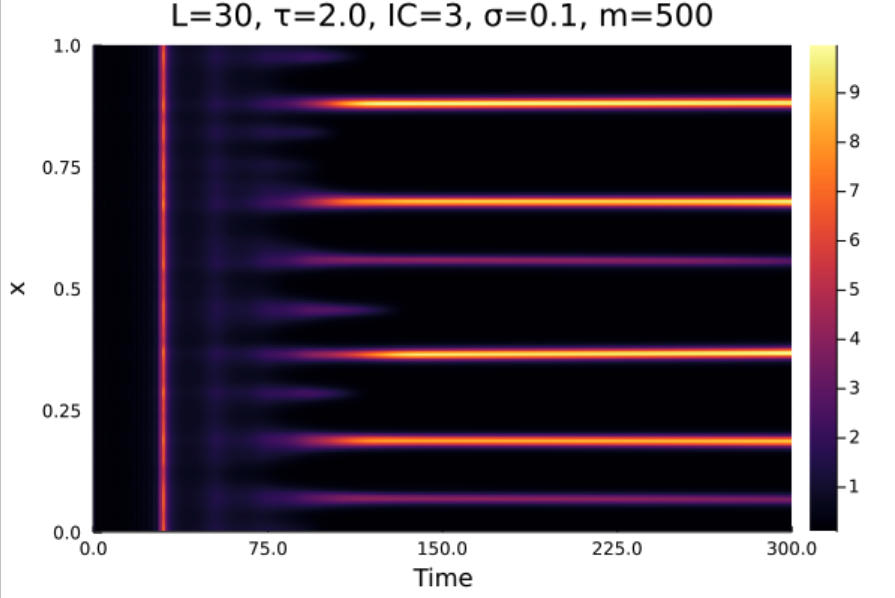
\includegraphics[width=6cm,height = 4.5cm]{l30t2ic3s1e1.png}
        \caption{}
        \label{}
    \end{subfigure}
    \hfill
    \begin{subfigure}[b]{0.45\linewidth}
        \centering
        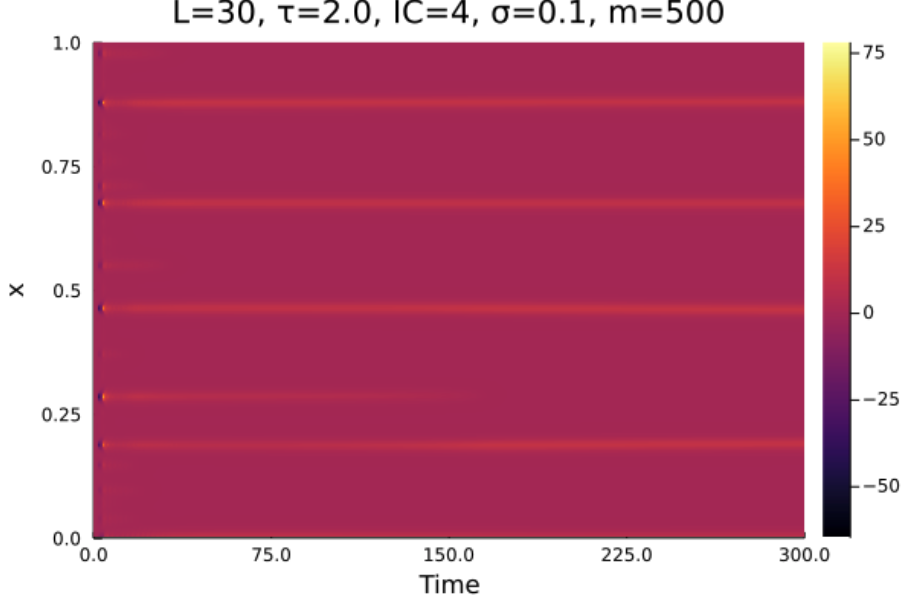
\includegraphics[width=6cm,height = 4.5cm]{l30t2ic4s1e1.png}
        \caption{}
        \label{}
    \end{subfigure}
    \caption{Comparison of IC3 with IC4}
    \label{}
\end{figure}


\newpage
\subsection{Neumann vs Mixed BCs}


\begin{figure}[H]
    \begin{subfigure}[b]{0.45\linewidth}
        \centering
        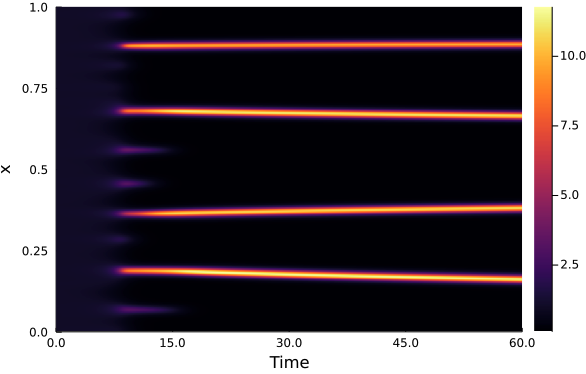
\includegraphics[width=6cm,height = 4.5cm]{t0neumannfixed.png}
        \caption{Neumann BCs}
        \label{}
    \end{subfigure}
    \hfill
    \begin{subfigure}[b]{0.45\linewidth}
        \centering
        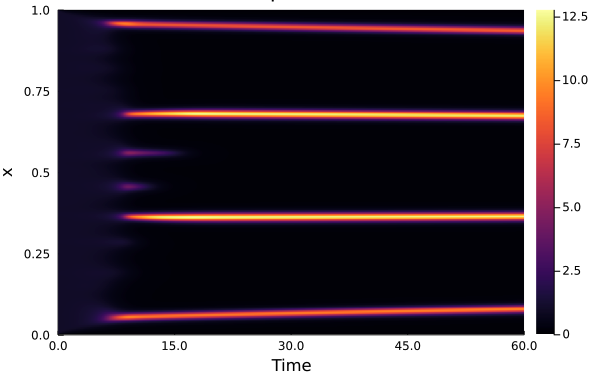
\includegraphics[width=6cm,height = 4.5cm]{t0mixedfixed.png}
        \caption{Mixed BCs}
        \label{}
    \end{subfigure}
    \caption{$\tau=0$}
\end{figure}
\begin{figure}[H]
    \begin{subfigure}[b]{0.45\linewidth}
        \centering
        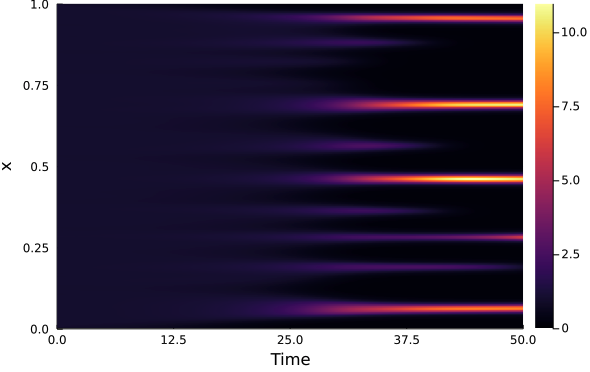
\includegraphics[width=6cm,height = 4.5cm]{t05neumannfixed.png}
        \caption{Neumann BCs}
        \label{}
    \end{subfigure}
    \hfill
    \begin{subfigure}[b]{0.45\linewidth}
        \centering
        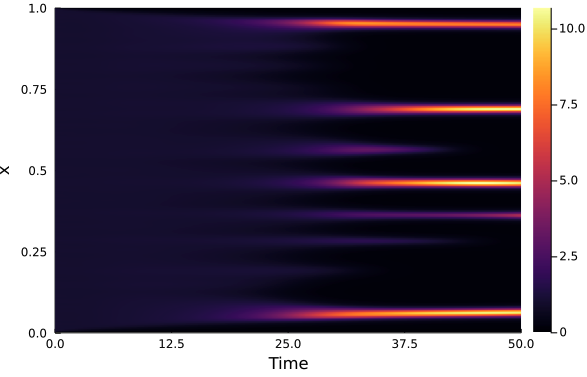
\includegraphics[width=6cm,height = 4.5cm]{t05mixedfixed.png}
        \caption{Mixed BCs}
        \label{}
    \end{subfigure}
    \caption{$\tau=0.5$}
\end{figure}
\begin{figure}[H]
    \begin{subfigure}[b]{0.45\linewidth}
        \centering
        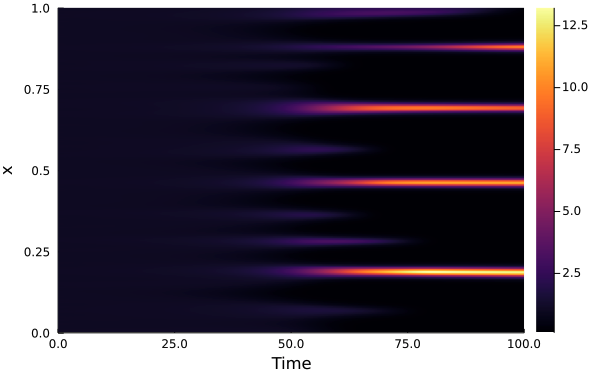
\includegraphics[width=6cm,height = 4.5cm]{t1neumannfixed.png}
        \caption{Neumann BCs}
        \label{}
    \end{subfigure}
    \hfill
    \begin{subfigure}[b]{0.45\linewidth}
        \centering
        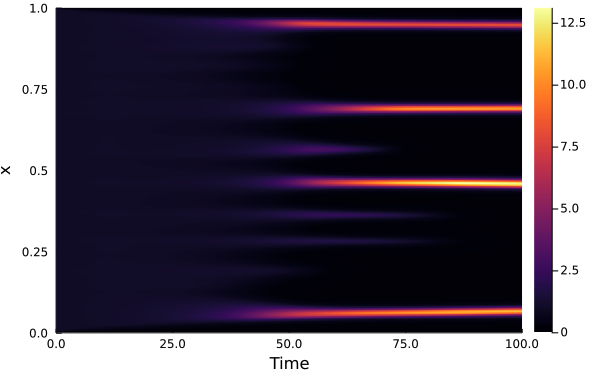
\includegraphics[width=6cm,height = 4.5cm]{t1mixedfixed.png}
        \caption{Mixed BCs}
        \label{}
    \end{subfigure}
    \caption{$\tau=1$}
\end{figure}
\begin{figure}[H]
    \begin{subfigure}[b]{0.45\linewidth}
        \centering
        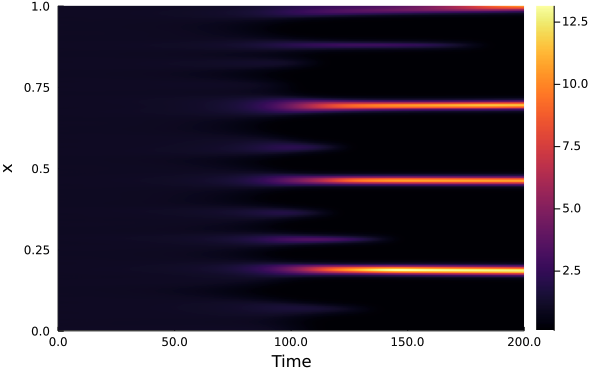
\includegraphics[width=6cm,height = 4.5cm]{t2neumannfixed.png}
        \caption{Neumann BCs}
        \label{}
    \end{subfigure}
    \hfill
    \begin{subfigure}[b]{0.45\linewidth}
        \centering
        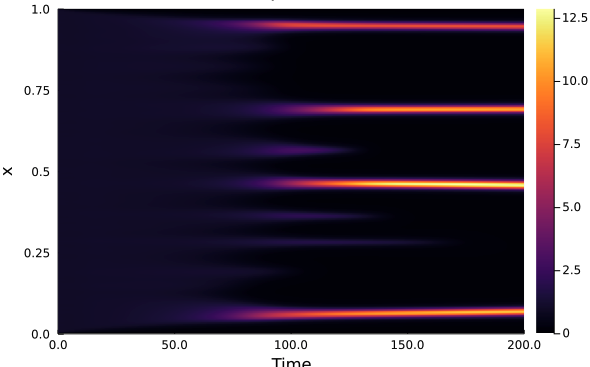
\includegraphics[width=6cm,height = 4.5cm]{t2mixedfixed.png}
        \caption{Mixed BCs}
        \label{}
    \end{subfigure}
    \caption{$\tau=2$}
\end{figure}
\begin{figure}[H]
        \begin{subfigure}[b]{0.45\linewidth}
            \centering
            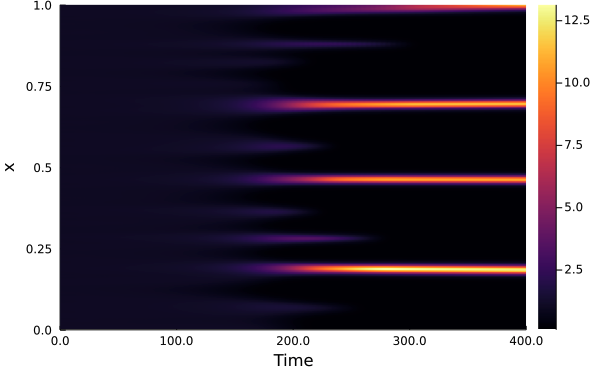
\includegraphics[width=6cm,height = 4.5cm]{t4neumannfixed.png}
            \caption{Neumann BCs}
            \label{}
        \end{subfigure}
        \hfill
        \begin{subfigure}[b]{0.45\linewidth}
            \centering
            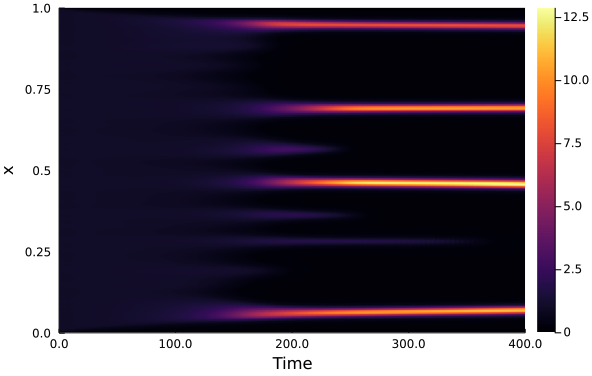
\includegraphics[width=6cm,height = 4.5cm]{t4mixedfixed.png}
            \caption{Mixed BCs}
            \label{}
        \end{subfigure}
        \caption{$\tau=4$}
    \end{figure}
    \begin{figure}[H]
        \begin{subfigure}[b]{0.45\linewidth}
            \centering
            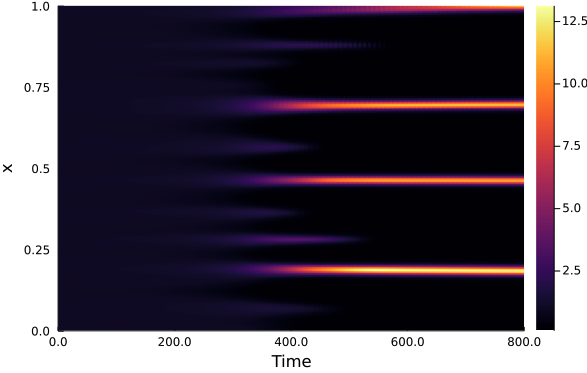
\includegraphics[width=6cm,height = 4.5cm]{t8neumannfixed.png}
            \caption{Neumann BCs}
            \label{}
        \end{subfigure}
        \hfill
        \begin{subfigure}[b]{0.45\linewidth}
            \centering
            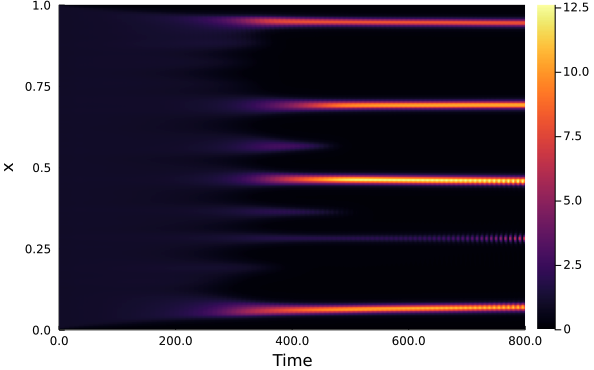
\includegraphics[width=6cm,height = 4.5cm]{t8mixedfixed.png}
            \caption{Mixed BCs}
            \label{}
        \end{subfigure}
        \caption{$\tau=8$}
    \label{}
\end{figure}



\end{document}
